\section{Results: What Accuracy a Macro Cell Allows}
\label{sec:results-error-scale}

% src: FINAL_REPORT.md §7.5 (pooled fit gamma 3.26, sigma 10.11 dB, R^2 0.204); pathloss_fit_summary.json comparison (fitted_gamma 3.264, fitted_sigma_db 10.106) and range_resolution (sigma_r 40.14 / 67.94 / 89.97 m at 56 / 95 / 126 m; 7.13 m at 10 m)
At the distances of the macro-cell study, RSS alone pins down range only to within tens of meters, and that sets the scale against which every error in the following sections should be read. Fitting Equation~(\ref{eq:path-loss}) to all $144{,}437$ macro-cell snapshots, with the antenna gain and antenna count of each device as controls, gives $\gamma = 3.26$ and a residual shadowing spread of $\sigma = 10.1\,\text{dB}$; range explains only $20\%$ of the variance in RSS. Dividing $\sigma$ by the gradient of Equation~(\ref{eq:rss-gradient}) turns this into the range uncertainty $\sigma_r$ implied by a single RSS reading: $40\,\text{m}$ at the 10th percentile of macro-cell range~($56\,\text{m}$), $68\,\text{m}$ at the median~($95\,\text{m}$), and $90\,\text{m}$ at the 90th percentile~($126\,\text{m}$). The same calculation gives $7\,\text{m}$ at $10\,\text{m}$ from the BS, the distance typical of the controlled grid. The two studies therefore differ not only in size but in how much a single RSS value says about distance, by roughly an order of magnitude. This is a ranging resolution and not a baseline: a model that ignored every measurement and always predicted the mean training position would be wrong by about $35\,\text{m}$ (Table~\ref{tab:reference-levels}).

Table~\ref{tab:reference-levels} sets this physical reference beside measured errors for both device groups, and beside the error of the simplest possible predictor, which always returns the mean training position: $35.3\,\text{m}$ for multi-antenna devices and $38.5\,\text{m}$ for single-antenna devices. A snapshot $k$-NN fingerprint, the classical approach, misses multi-antenna devices by $23\,\text{m}$ on average and single-antenna devices by $46\,\text{m}$, which for single-antenna devices is worse than the constant guess. The trained models do considerably better for multi-antenna devices: over $20$ user splits XGBoost is $47\%$ below the constant guess at $h=0$ and $56\%$ below it at $h=5$. For single-antenna devices they do not: XGBoost is $6\%$ below it at $h=0$ and $5\%$ at $h=5$, and the two groups remain about $20\,\text{m}$ apart in every model.

\begin{table}[h]
  \centering
  \caption{Reference error levels in the macro-cell study, per device group. Measured errors are means over five seeds, and the constant-guess errors means over $20$ seeds; neural-model errors are optimistic because their stopping epoch was chosen on the test users. The ranging resolution is a standard deviation, not an error.}
  \label{tab:reference-levels}
  \small
  \begin{tabular}{@{}lrr@{}}
    \toprule
    Reference & Multi-antenna & Single-antenna \\
    \midrule
    Constant guess (mean training position) & $35.3\,\text{m}$ & $38.5\,\text{m}$ \\
    RSS ranging resolution $\sigma_r$ at median range & $68\,\text{m}$ & $68\,\text{m}$ \\
    \midrule
    $k$-NN, $h=0$ & $23.4\,\text{m}$ & $46.2\,\text{m}$ \\
    XGBoost, $h=0$ & $18.8\,\text{m}$ & $35.8\,\text{m}$ \\
    XGBoost, $h=5$ & $15.7\,\text{m}$ & $35.8\,\text{m}$ \\
    Best of seven models, $h=5$ & $15.5\,\text{m}$ & $34.5\,\text{m}$ \\
    \bottomrule
  \end{tabular}
\end{table}
% src: constant guess: followup_2026_10/naive_baseline/*/naive_position_baseline_summary.json (20 seeds: multi 35.27+-0.54, single 38.50+-1.21, all 35.67); XGBoost vs guess: followup_2026_10/uniform_nlos snap/full means 18.74/15.59 multi, 36.33/36.51 single; row 2 as above; rows 3-6: seed_repeats_all_models_summary.json per_config (knn_h0 23.38/46.17; xgboost_h0 18.81/35.84; xgboost_h5 15.65/35.77; best h5: cnn_attn multi 15.45, mask_aware_cnn single 34.52)

% src: diagnostics_2026_10/baseline_uniform_nlos summary per_seed.xgboost.{snap,full} (5 seeds): within_5m/10m/20m, p50, p90; errors_first_seed.npz (figure, seed 42)
The two groups are clearly separated in the error distribution, though not disjoint~(Figure~\ref{fig:error-cdf}): their error histograms overlap by $52\%$ with history and $63\%$ without in the plotted split. With five steps of history, XGBoost places $34\%$ of multi-antenna predictions within $10\,\text{m}$ of the true position and $71\%$ within $20\,\text{m}$, with a median error of $13.7\,\text{m}$ and a 90th percentile of $29.5\,\text{m}$. For single-antenna devices the corresponding fractions are $7\%$ and $21\%$, the median is $34.7\,\text{m}$, and the 90th percentile is $59.1\,\text{m}$. Fewer than $12\%$ of multi-antenna predictions and $2\%$ of single-antenna predictions fall within $5\,\text{m}$.

\begin{figure}[h]
  \centering
  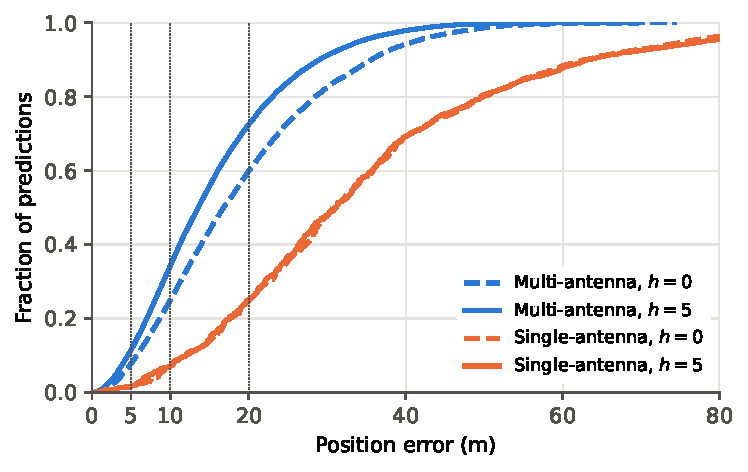
\includegraphics[width=0.7\textwidth]{fig_error_cdf}
  \caption{Distribution of position error per device group, XGBoost without history~($h=0$, dashed) and with five steps of history~($h=5$, solid), macro-cell study, one seed. Dotted lines mark $5$, $10$ and $20\,\text{m}$.}
  \label{fig:error-cdf}
\end{figure}
% src: figure_scripts/make_figures_diagnostic.py error_cdf(); diagnostics_2026_10/baseline_uniform_nlos/errors_first_seed.npz

% src: diagnostics_2026_10/baseline_uniform_nlos summary per_seed.xgboost.{snap,full} radial_mean / tangential_mean (5-seed means: multi h5 14.12 / 4.60; single h5 20.13 / 25.29); radial share = r^2/(r^2+t^2) as in error_decomposition.py; followup_2026_10/uniform_nlos summary.xgboost.snap.single.shape (20 seeds: radial share 0.41+-0.02, range_corr 0.51+-0.06, radial_bias -9.73) and full.multi.shape radial_rms 17.45
The two groups also fail in different directions. Splitting each error into its component along the line to the BS, the radial or range error, and the component across it, the tangential or cross-range error, shows that multi-antenna devices are limited by range. With history, their mean radial error is $14.1\,\text{m}$ against a tangential error of $4.6\,\text{m}$, so $90\%$ of their error variance lies along the line to the BS. That radial error, $17.5\,\text{m}$ in root-mean-square terms, is about four times smaller than the $68\,\text{m}$ standard deviation of a single-reading range estimate, so the models extract considerably more range information than a path-loss inversion. Single-antenna devices fail differently. Their tangential error of $25.3\,\text{m}$ exceeds their radial error of $20.1\,\text{m}$, and about $60\%$ of their squared error is tangential, which is the distance-ring ambiguity of Section~\ref{subsec:ambiguity-hypothesis} observed. But they are not placed at the right distance: their radial error is larger than that of multi-antenna devices, the predicted range correlates only $0.51 \pm 0.06$ with the true range, and predictions are pulled toward the BS by about $10\,\text{m}$ on average. Over $20$ splits these devices are only $5$ to $6\%$ better than the constant guess of Table~\ref{tab:reference-levels}.

% src: diagnostics_2026_10/baseline_uniform_nlos summary per_seed.xgboost.{snap,full}.groups.*.range_bins (5-seed means; multi h0 21.3/21.2/14.5/28.6, h5 11.1/17.2/12.9/23.1; single h0 31.9/30.4/37.5/41.0; mean test samples per band, single: 163/1318/2549/728)
Error does not simply grow with distance from the BS~(Figure~\ref{fig:error-by-range}). For multi-antenna devices the band from $80$ to $120\,\text{m}$, which holds about half of the test samples, has the smallest error, while both the nearest band and the farthest have larger errors. The nearest band is also where history makes the largest difference, cutting the mean error from $21.3$ to $11.1\,\text{m}$. Single-antenna error rises from about $30\,\text{m}$ within $80\,\text{m}$ of the BS to about $40\,\text{m}$ beyond $120\,\text{m}$, and history changes it in none of the bands. Only about $160$ single-antenna test samples per split fall within $40\,\text{m}$ of the BS, so that band is the least certain.

\begin{figure}[h]
  \centering
  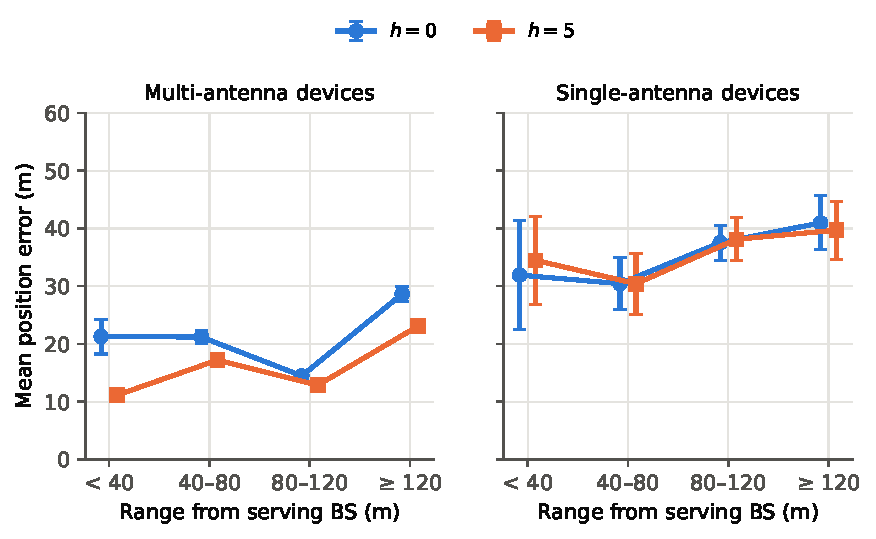
\includegraphics[width=0.85\textwidth]{fig_error_by_range}
  \caption{Mean position error by range from the serving BS, per device group, XGBoost without and with history, macro-cell study. Means over five seeds; bars are $95\%$ confidence intervals across seeds.}
  \label{fig:error-by-range}
\end{figure}
% src: figure_scripts/make_figures_diagnostic.py error_by_range()

% src: FINAL_REPORT.md §7.5 ("eight differences": 784 vs 9,216 m^2; ~1,600 vs 178 samples per cell; seen vs unseen users)
The gap between the controlled grid's sub-meter errors and the macro cell's tens of meters follows from these references rather than from a failure of the models. Beyond the order-of-magnitude difference in what one RSS reading says about range, the macro cell covers twelve times the area, offers about nine times fewer training samples per grid cell, and tests on users the model has never seen. Because the two device groups fail in such different ways, the effect of history has to be measured on each of them separately.
